\documentclass{standalone}
\usepackage{pgfplots}
\usepgfplotslibrary{groupplots, fillbetween}
\usetikzlibrary{patterns}
\pgfplotsset{compat=1.6}
\pgfplotsset{solid-dot/.style={only marks,mark=*}}
\pgfplotsset{hollow-dot/.style={fill=white,only marks,mark=*}}

\begin{document}

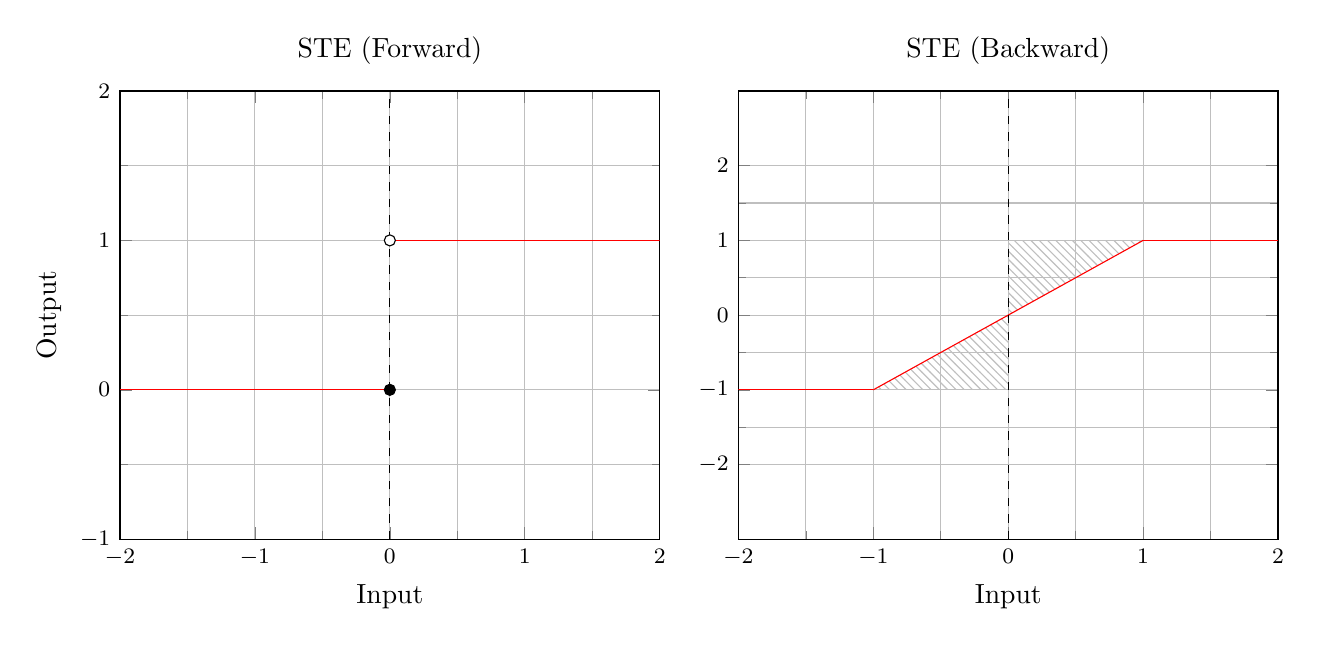
\begin{tikzpicture}
  \begin{groupplot}[group style={group size= 2 by 1},
    grid=both, minor tick num=1,
    xmin=-2, xmax=2,
    tick label style={font=\footnotesize},
    xlabel={Input}]
    \nextgroupplot[ylabel={Output}, title={STE (Forward)},
    ymin=-1, ymax=2]
    \addplot[domain=-2:0,red] {0};
    \addplot[domain=0:2,red] {1};
    \draw[dashed] (axis cs:0,-1) -- (axis cs:0,2);
    \addplot[hollow-dot] coordinates{(0,1)}; 
    \addplot[solid-dot] coordinates{(0,0)}; 
    \nextgroupplot[title={STE (Backward)}, ymax=3, ymin=-3, ytick distance = 1,
    ytick={-2, -1, 0, 1, 2}] 
    \addplot[domain=-2:-1,red] {-1};
    \addplot[domain=1:2,red] {1}; 
    \addplot[domain=-1:1,red,name path=A] {x};
    \addplot[dashed] coordinates {(0,-3)(0,3)};
    \path[name path=axis] (axis cs:0,-1) -- (axis cs:0,0);
    \path[name path=axis-next] (axis cs:0,1) -- (axis cs:0,0);
    \addplot[pattern=north west lines, pattern color=gray!50!white] fill between[of=A and axis];
    \addplot[pattern=north west lines, pattern color=gray!50!white] fill between[of=A and axis-next];
  \end{groupplot}
\end{tikzpicture}

\end{document}